\documentclass{template/openetcs_article}
% Use the option "nocc" if the document is not licensed under Creative Commons
%\documentclass[nocc]{template/openetcs_article}
\usepackage{url,longtable}
\graphicspath{{./template/}{.}{./images/}}
\begin{document}
\frontmatter
\project{openETCS}

%Please do not change anything above this line
%============================
% The document metadata is defined below

%assign a report number here
\reportnum{OETCS/WP4/D4.2aV2.1}

%define your workpackage here
\wp{Work-Package 4: ``Verification and Validation''}

%set a title here
\title{Preliminary safety Evaluation Criteria}

%set a subtitle here
\subtitle{Latex Document - Review Version}

%set the date of the report here
\date{May 2013\\Revised June 2013}

%define a list of authors and their affiliation here

\author{Jan Welte}

\affiliation{Technische Universität Braunschweig\\
  Institute for Traffic Safety and Automation Engineering \\
  Langer Kamp 8 \\
  38118 Braunschweig\\
  Germany}

% define the coverart
\coverart[width=350pt]{openETCS_EUPL}

%define the type of report
\reporttype{Output for secondary tool evaluation}


\begin{abstract}
%define an abstract here
  This document presents an overview of the safety related evaluation criteria used within the openETCS document structure and based on this derives evaluation criteria for the choice of suitable tools and methods for all safety design activities which have to be performed during the openETCS development process. These criteria are based on the safety design activities required in D2.6 and the general concept for an openETCS safety design process. 
\end{abstract}

%=============================
%Do not change the next three lines
\maketitle
\tableofcontents
\listoffiguresandtables
\newpage
%=============================

% The actual document starts below this line
%=============================


%Start here

\section{Safety Process}

The EN50128 standard defines safety as the ``freedom from unacceptable levels of risk of harm to people" \cite{EN50128:2011}, which shows that the safety approach required by the CENELEC standards is risk-based. As the risk is defined as the ``combination of the rate of occurrence of accidents and incidents resulting in harm (caused by a hazard) and the degree of severity  of that harm" \cite{EN50128:2011} this approach is based on a probabilistic understanding of event occurrence. The overall relations between all these safety-related terms used to define the safety properties, characteristics and quantities are outlined by the Risk-Genesis-Model of Schnieder, which is shown in the following figure \ref{fig:Risiko-Genese-Modell-eng}.

\begin{figure}[htbp]
\centering
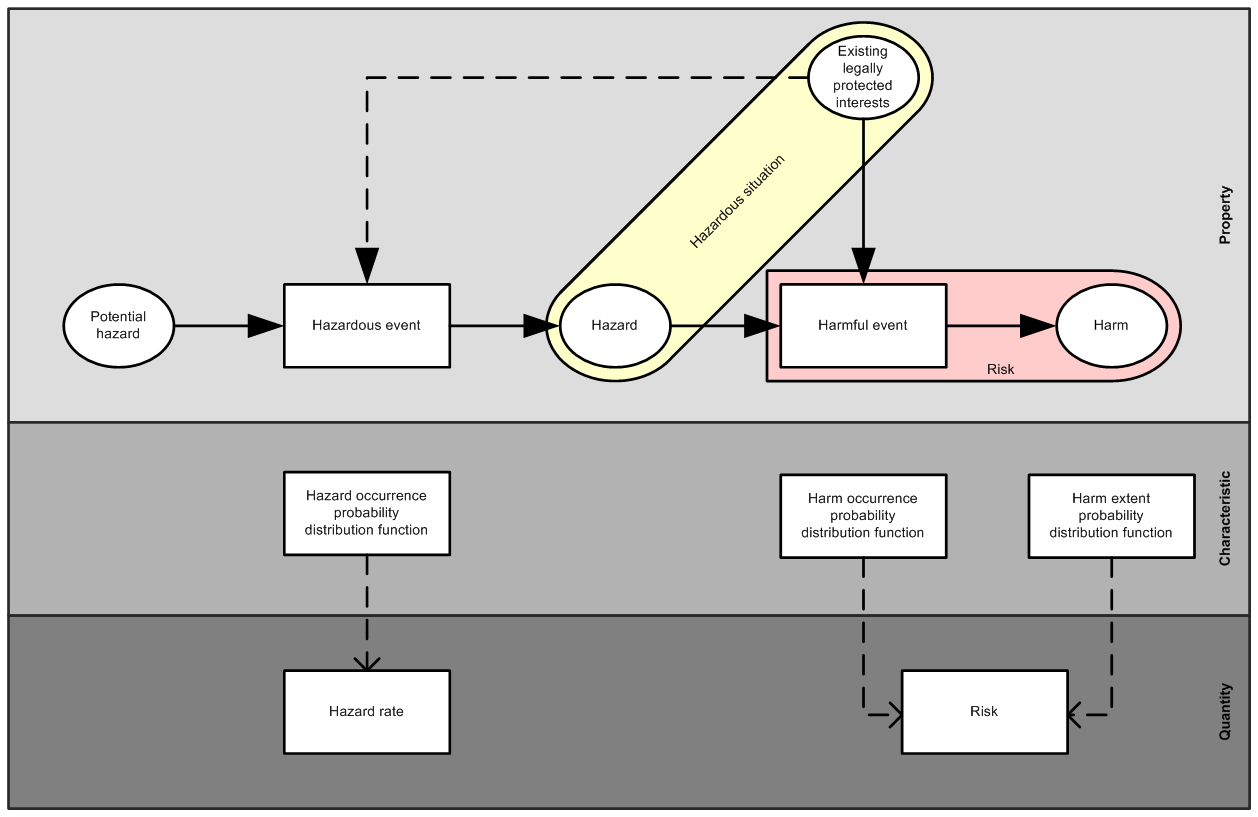
\includegraphics[width=0.7\linewidth]{bld_2013-06-19_Risiko-Genese-Modell-eng-2-0_jw}
\caption{Risk-Genesis-Model showing the relations between the safety-related terms \cite{Schnieder.2010}}
\label{fig:Risiko-Genese-Modell-eng}
\end{figure}

This demonstrates that the first step is to define the system properties, specifically identifying the harms and their related hazardous situations. This has to be performed during a system hazard analysis. Afterwards the respective properties have to be determined by assessing the risk concerning the identified hazards. Based on this work safety integrity levels can be assigned to all system functionalities which are then allocated during the design to certain parts of the operational equipment. As this work is closely related to all design decisions, it has to be done iteratively for all abstraction levels during the system design. 

\begin{figure}[htbp]
\centering
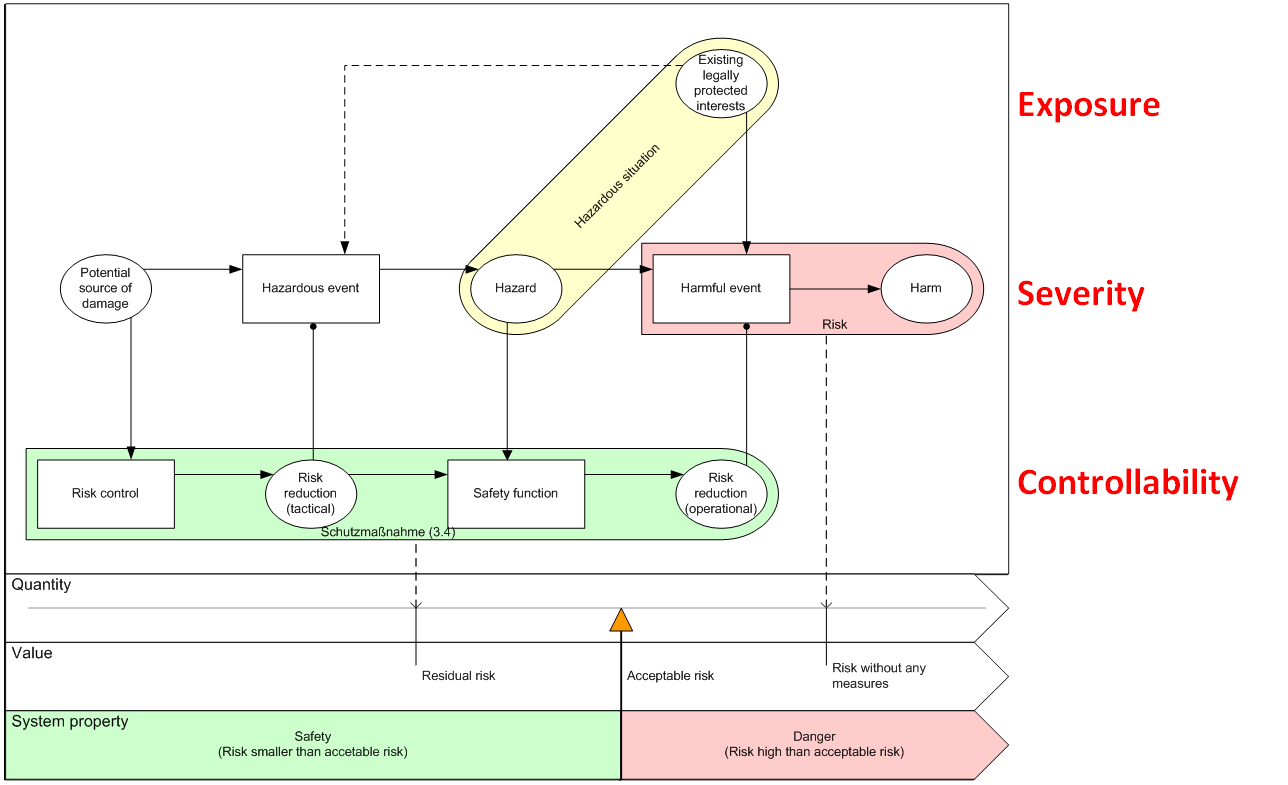
\includegraphics[width=0.7\linewidth]{bld_2013-06-19_Risk-control-modell_1-0_jw}
\caption{Risk control process \cite{Schnieder.2013}}
\label{fig:Risk-control-modell-eng}
\end{figure}

The safety integrity level represented the acceptable risk for every part of the system. The risk control process as it is presented in figure \ref{fig:Risk-control-modell-eng} is then performed to ensure that the safety integrity levels are reach by every part of the system.

Since software itself does not fails in the way technical equipment does the specific software safety integrity level represent a qualitative measure with respect to the required degree of correctness for the software functionality than a qualitative value for the likelihood of failing. To reach the needed degree of correctness for the software various design, verification and validation methods are required corresponding to the assigned software safety integrity level. This process leads to safety requirements which have to be implemented in the software design as well as verified and validated. Respectively the EN50126 describes the safety design process as a series of safety tasks for each life cycle phase. This task are related to a number of safety artifacts which are created, used and adapted over time through the different safety design activities.

\subsection{Safety artifacts}

Since all safety design activities are based on the system development activities all system design artifacts are part of the safety design process. Therefore, the following design artifacts of the CENELEC standard development process build the basis for all safety artifacts:

\begin{itemize}
\item System Concept
\item System Requirements Specification
\item Software Requirement Specification
\item Software Architecture Specification
\item Software Design Specification
\item Software Module Design Specification
\item Software Source Code
\end{itemize}

The main safety artifacts are those which are set-up to build the reference for the safety-related aspect during the system development, which are continuously evolved during the design phases. Correspondingly the safety design process has to create artifacts to demonstrated that all safety and quality-related requirements included in the system design. Respectively the following artifacts are created during the safety design process:

\begin{itemize}
\item System Safety Plan
\item Software Quality Assurance Plan
\item Hazard Log
\item System Safety Requirement Specification
\item Safety Case
\end{itemize} 

This artifacts have to be managed over the development process. Since all safety requirement have to be verified and validated there is likewise a close to all Test and Validation Reports.

\subsection{Safety design activities}
\label{safetyactivities}
The safety design activities set-up or evolve the safety artifacts in relation to the different design artifacts. The following safety design activities are required according to the EN 50128:

\begin{itemize}
\item Preliminary Hazard Analysis
\item Establish Safety Plan
\item System Hazard and Risk Analysis
\item Risk Assessment
\item Specification of System Safety Requirements
\item Define Safety Related Functional Requirements
\item Specify Sub-System and Component Safety requirements
\item Implement Safety Plan
\item Verify System, Sub-System and Component Safety requirements
\item Validate System Safety Requirements
\item Establish Safety Case
\end{itemize}

Overall the safety design activities have to be performed in close relation to the overall verification and validation activities as these have to verify and validate all safety requirements and their results become part of the safety plan.


\subsection{OpenETCS safety design process}

The presented CENELEC standard safety artifacts and activities are always related to the overall system development. Since the openETCS development process just describes the development of the on-board unit software for ETCS additional system informations are needed for the openETCS safety design process. These are mainly the following two parts of the CCS TSI:

\begin{itemize}
\item UNISIG SUBSET-026	System Requirements Specification 	(Version 3.3.0)
\item UNISIG SUBSET-091 Safety Requirements for the Technical Interoperability of ETCS in Levels 1 and 2 	(Version 3.2.0)
\end{itemize}

In relation to SUBSET-91 further documents should be considered:

\begin{itemize}
\item Part of TSI Annex A
	\begin{itemize}
	\item SUBSET-036
	\item SUBSET-037
	\item SUBSET-040
	\item SUBSET-041
	\item SUBSET-098
	\end{itemize}
	
\item Not part of TSI Annex A
	\begin{itemize}
	\item SUBSET-039
	\item SUBSET-078
	\item SUBSET-079
	\item SUBSET-080
	\item SUBSET-081
	\item SUBSET-088
	\end{itemize}
\end{itemize}

From these documents the Preliminary Hazard Analysis and the System Safety Goals have to be derived which are needed as the starting point for the openETCS safety design process. Based on these information a subsystem hazard and risk analysis for the openETCS scope can be performed which set-up the openETCS hazard log. Based on these results the openETCS safety requirements will be specified, which are then further developed to functional requirements. During the development these requirements are adopted if necessary for the different abstraction levels from the high level model down to the source code. This is done using corresponding safety backlogs, which are the reference for the safety requirement verification. Altogether the source code has to be validated against all safety requirements to demonstrated, that software faults can not cause any harm. The safety case has to present all needed documentation.
 
The main task of the openETCS safety design process and the interactions with the design process are shown in figure \ref{fig:WholeSafetyProcess}.

\begin{figure}[htbp]
\centering
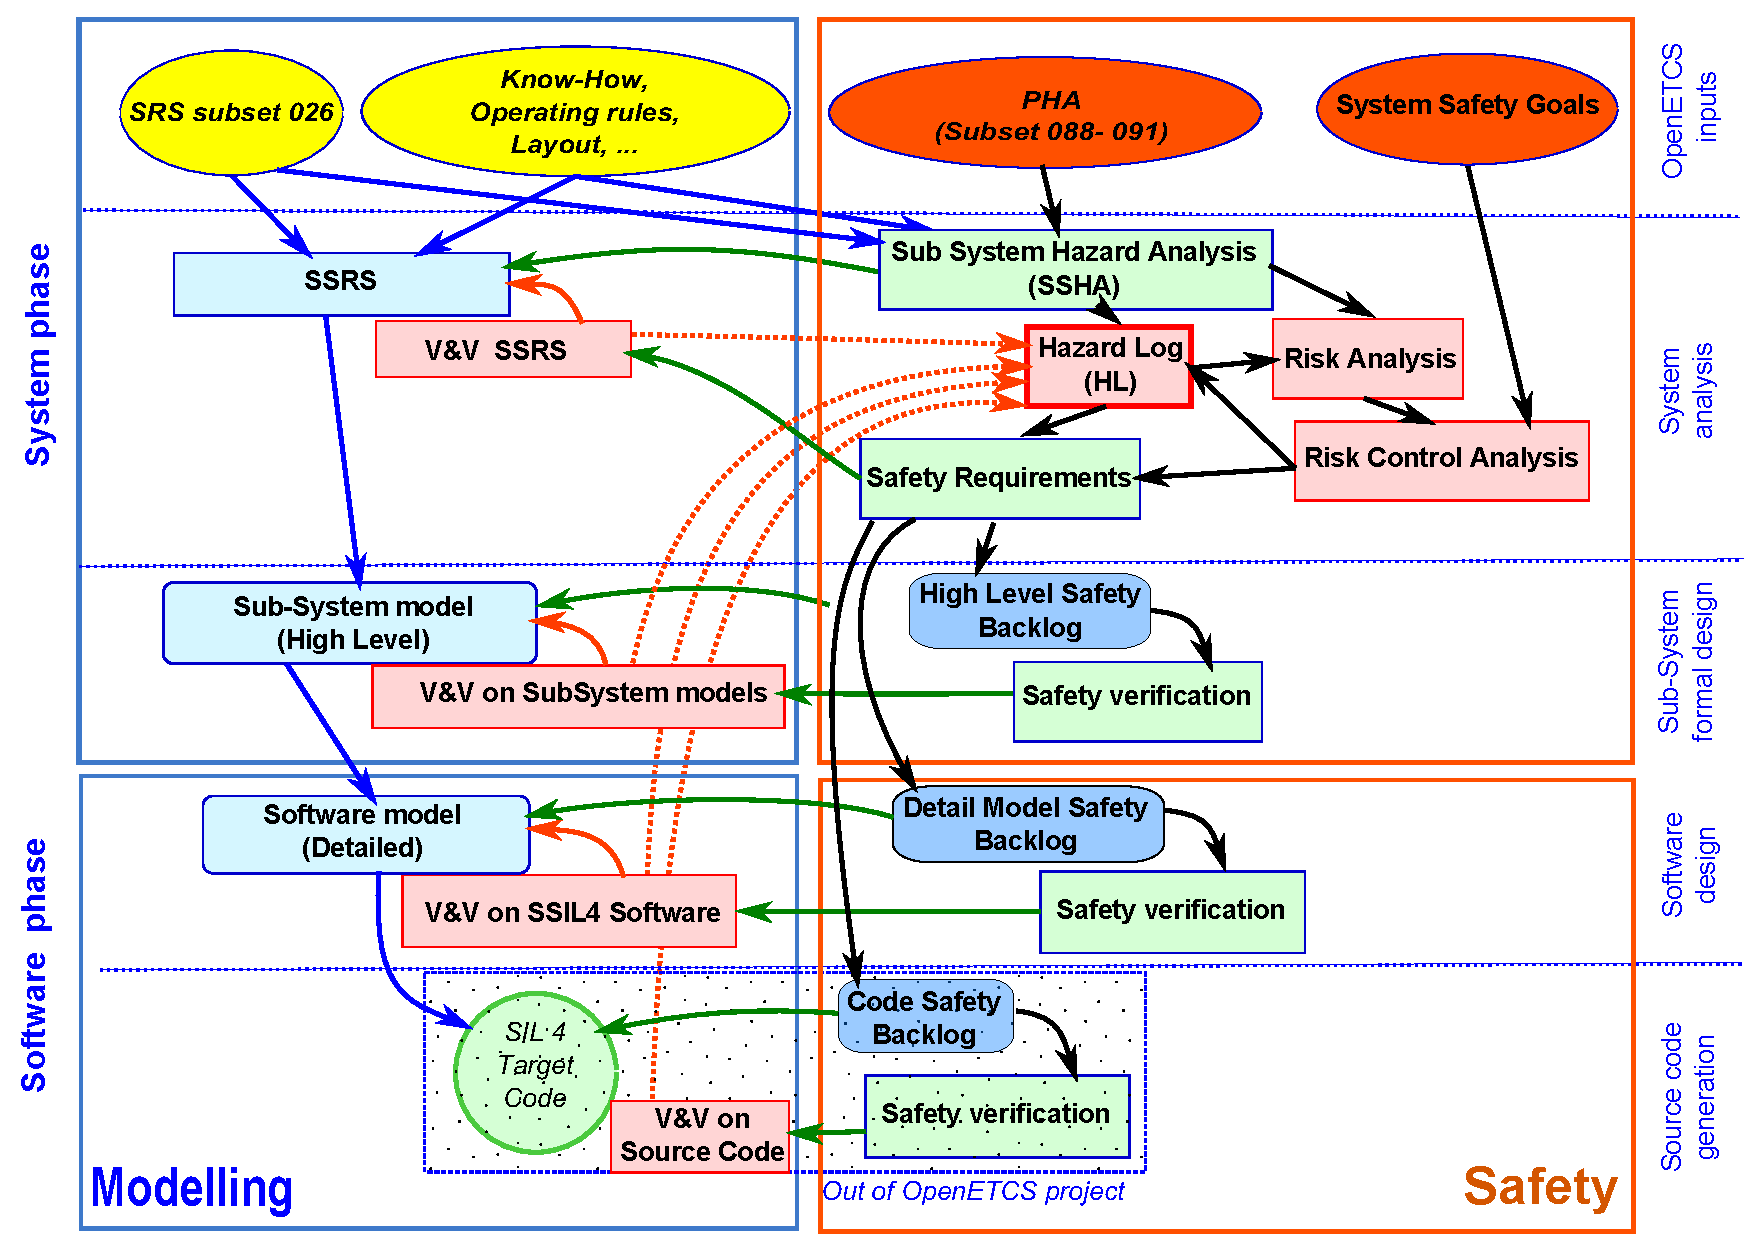
\includegraphics[width=0.8\linewidth]{WholeSafetyProcess}
\caption{OpenETCS Safety Design Process}
\label{fig:WholeSafetyProcess}
\end{figure}

The openETCS safety design process will be specified more detailed in the safety plan. Correspondingly, the main safety artifacts and safety design activities which have to be handled during the openETCS safety design process are shown in table \ref{tab:openETCS-Safety-artifacts} and \ref{tab:openETCS-Safety-activities}.

% Table generated by Excel2LaTeX from sheet 'Artifact Categorization'
\begin{table}[htbp]
  \centering
  \caption{Main openETCS safety design process artifacts}
    \begin{tabular}{r|p{8cm}|p{4cm}}
    \textbf{Abbreviation} & \textbf{Safety Artifact} & \textbf{Degree of Formalisation}\\
    \hline
    Safety Req & Safety Requirements: list of all requirements which have to be respected during the system development to reach the safety goals & Informal/ Semi-Formal / Formal \\
    HL    & Hazard Log: List of identified hazards and its associated risk classification as well as information concerning the risk control & Informal \\
    SP    & Safety Plan: Document which specifies all activities, resources and events to ensure that the source code will satisfy all relevant safety requirements & Informal \\
    SC    & Safety Case: Documentation which demonstrates that the used development process and the resulting source code fulfil all safety requirements & Informal \\
    CSB   & Code Safety Backlog: list of requirements/ properties to be implemented inside the dM derived from  the HL (and the dMSB) & Semi-Formal/ Strictly-Formal \\
    dMSB  & Detailed Model Safety Backlog: list of requirements/ properties to be implemented inside the dM derived from the HL (and  the hLSB) & Semi-Formal/ Strictly-Formal \\
    hLSB  & High Level Safety Backlog: list of requirements/ properties to be implemented inside the hM derived from the HL & Informal/ Semi-Formal \\
    \end{tabular}%
  \label{tab:openETCS-Safety-artifacts}%
\end{table}%

\begin{table}[htbp]
  \centering
  \caption{Main openETCS safety design process activities}
    \begin{tabular}{p{4cm}|p{6cm}|p{4cm}} 
 \textbf{Safety Design Activity} & \textbf{Input Artifact(s)} & \textbf{Output Artifact(s)}  \\ \hline
 Establish Safety Plan & QA-Plan + Project documentation (FPP, …) & Safety Plan \\
 Preliminary Hazard Analysis (PHA) & Mainly SUBSET-91(+SUBSET-88) &  Safety Goals + Safety Acceptance Criteria +  PHA report\\ 
 Sub-System Hazard and Risk Analysis (SSHA) & Safety Goals and Acceptance Criteria + SSRS + additional design and architecture specification + additional user constraints  & Hazard Log (incl. Hazards and Safety Functions) \\ 
  Specification of Sub-System Safety Requirements & SUBSET-26 + SUBSET-91 + Hazard Log  & Safety Requirement Specifications \\ 
 Update Hazard Log and corresponding Sub-System Safety Requirements & Verification Reports + Test Cases & Hazard Log + Sub-System Safety Requirements \\
 Specify model specific Requirements & SSRS + Safety Requirement Specification & Safety Plan + Model Backlogs\\
 Verify Safety Requirements & Models + Safety Requirements + Model Backlogs & Verification Report + Verification report \\
 Validate Safety Requirements & Source Code + Safety Requirements & Validation Report + Validation report \\
 Establish Safety Case & V and V Plan + Safety Plan + all requirements and specifications + V and V Reports & Safety Case \\ 
 
\end{tabular}  
  \label{tab:openETCS-Safety-activities}%
\end{table}%

\subsection{Safety design process supporting tools}

Supporting software tools are needed to handle the safety artifacts and to some degree to more efficiently perform the safety design activities. As some safety artifacts like the safety requirement specifications and the safety backlogs are closely related to design artifacts the same tools can be used. Especially all requirements should be handled by one tool to ensure full traceability and provide one main interface for the verification and validation activities.

Depending on the methods used for hazard and risk analysis appropriate tools are needed to perform the analysis, collect the hazards and associated risks in the hazard log and to evaluated possible risk control measures. Thereby, traceability has to be guaranteed between all activities.

Since the safety plan and safety case provide the basis for the safety approval the tools used to generated these artifacts should help to generate a consistent argumentation and efficiently collect the data needed to provide evidence. Respectively, interfaces to manage documents and automatically generate reports would be helpful functionalities.

\newpage

\section{Evaluation Criteria}

The safety design process has to ensure and demonstrated that the development process in general and the specific source code provide adequate protection against all relevant hazards. Therefore the safety design process and the supporting tools have to be linked to the design process and especially the requirement handling and verification and validation activities. Thereby traceability between safety artifacts and design artifacts is the main issue.

\subsection{Safety Design Process}

The safety design process and the resulting documentation constitute the main documents for the system approval, as it is required by European and national law to do everything reasonable expectable to prevent harm. Accordingly the CENELEC standards build the common technical rules for the development process. The Common Safety Methods present a concept based on the EN50126 how the risk evaluation and management has to be performed. 

Therefore the main references concerning the safety design process are the CENELEC standards, mainly the EN50126 on how the safety aspects have to be handled as part of the RAMS management over the development process. The overall risk evaluation concept is also defined at this point. The specific concerning the safety case preparations are defined in the EN50129 including the Safety Integrity Level concept. 

Therefore the overall safety management process has to be followed during the openETCS project, as far as it is concerning the scope of openETCS. Therefore the following table \ref{tab:Safety Process Requirements} presents a first list of relevant requirements:

\begin{table}[htbp]
  \centering
  \caption{CENELEC Safety Process Requirements}
    \begin{tabular}{r|r|r}
    Standard & Section & Titel \\
    \hline
     EN 50126 & 4 & Railway RAMS  \\ 
    EN 50126 & 6 & RAMS lifecycle \\
     EN 50128 & Table A.3 & Software Error Effect Analysis\\
    EN 50129 & 5.3 & Evidence of safety management \\
    EN 50129 & Annex A & Safety Integrity Levels \\
    EN 50129 & Annex B & Detailed technical requirements \\
    \end{tabular}%
  \label{tab:Safety Process Requirements}%
\end{table}%

\subsection{Supporting tools}

All tasks of the safety design process have to be supported by suitable tools, which are able to handle the artifacts. As the openETCS project wants to use FLOSS tools, this is also one important evaluation criteria for all tools of the safety design process. As it has been demonstrated in subsection \ref{safetyactivities} most safety design activities have to deal with in- and output from design artifacts, therefore the tools shall be able to interact with those data formats chosen for the specific design artifacts. Overall the safety design process tools should be integrated into the tool chain as far as possible.  

In addition some tools needed to support the safety design process basically provide the same functionality as it is used during the design or the verification and validation process. If there is no specific need to use different tools to avoid common failures, the same tools shall be used for the same functionalities to reduce interfaces.

Table \ref{ToolEvalCrit} gives an overview about the needed supporting tools and the main evaluation criteria for each of the tools.



  
    \begin{longtable}[htbp]{p{4cm}|p{5cm}|p{5cm}}
    
    \caption{Supporting tools and associated evaluation criteria}   
    \label{ToolEvalCrit} \\
    
          \textbf{Evaluation Criteria} & \textbf{Description} & \textbf{Evaluation Criteria} \\
            \hline
        \endfirsthead
        
        \textbf{Evaluation Criteria} & \textbf{Description} & \textbf{Evaluation Criteria} \\
        \hline
        \endhead
        
        \hline\multicolumn{3}{r}{\textit{Continued on the next page}}\\\hline
        \endfoot
        \hline
        \endlastfoot
    
    Text Editor & Editor to write mainly textual documents e.g. Safety Plan,  & \begin{itemize}
    \item Usability
    \item Open formats
    \item Tool chain integration
        \end{itemize}
     \\ 
     Modelling (and Analysis) tool for top-down Hazard Analysis & To identify potential hazards a top-down system analysis will be performed. To do this methods like FTA or STAMP use different kinds of modelling tools to systematically identify hazards in the system structure and behaviour. To efficiently use this methods a modelling editor with limited functionalities to analyse the model is needed.  & \begin{itemize}
         \item Simple Usability
         \item Modelling (and Analysis) functionality depending on method
         \item Vertical tool chain integration (import system information/ export hazard information)
         \item Traceability to SRS and SSRS
             \end{itemize} \\ 
     Modelling (and Analysis) tool for bottom-up Hazard and Risk Analysis & To identify potential hazards and to estimate the risk a bottom-up system analysis will be performed. To do this methods like FMEA or HAZOP use different kinds of systematic approaches to evaluated the system structure and its behaviour. To efficiently use this methods a modelling editor with limited functionalities to analyse the model is needed.  & \begin{itemize}
              \item Simple Usability
              \item Modelling (and Analysis) functionality depending on method
              \item Vertical tool chain integration (import system information/ export hazard and risk information)
              \item Traceability to SRS and SSRS
                  \end{itemize} \\ 
                  
     Database for Hazard Log & The hazard log is the central artifact to collect all identified hazards and their associated risks as well as potential risk control measures. A database tool is needed to store these hazards while providing the needed traceability information to retrace their correct identification and evaluation. & \begin{itemize}
                        \item Simple Usability
                        \item Proper Versioning system 
                        \item Easy ability for Queries
                        \item Horizontal tool chain integration
                        \item Traceability to Hazard and Risk Analysis and Safety Requirements
                        \item Generation of documentation
                            \end{itemize} \\
                  
     Database for Safety Requirements & As the safety requirements have to be defined based on the risk control measures chosen based on the hazard and risk analysis, these have to be stored and handled as all other requirements. & \begin{itemize}
                   \item Simple Usability
                   \item Proper Versioning system 
                   \item Easy ability for Queries
                   \item Horizontal and vertical tool chain integration
                   \item Traceability to Hazard Log, all design, verification and validation artifacts
                   \item Generation of documentation
                       \end{itemize} \\  
     Tools for safety requirement verification and validation & Tools equivalent to verification and validation tools to handle the safety requirements & \begin{itemize}
                        \item Simple usability
                        \item Efficient performance
                        \item Vertical tool chain integration
                        \item Traceability to safety requirements
                        \item Ability to provide T2 (or T3) tool qualification 
                        \item Automatic generation of documentation
                            \end{itemize}\\
     Safety Case management tool & To develope and manage the safety case over time from the generic concept to the specific documentation a tool is needed. This tool has to help to develope a consisten generic argumentation chain and to link this to the actual documents. Thereby the information concerning the documents should be provided mostly automatically to avoid inconsistencies. & \begin{itemize}
                   \item Simple Usability
                   \item Modelling  functionality for safety case structure
                   \item Linking to versioning and configuration systems
                   \item Automatic document generatio
                       \end{itemize}   \\ 
    \end{longtable}%
 


\section{Conclusion}

This document presents a general overview about the safety design process as it will be implemented in the openETCS project and which references have to be respected. This plan will be developed further in the actual safety plan. As most safety design activities are closely related to design, verification and validation activities more details will be defined as these processes are refined.

Based on this safety design process concept evaluation criteria mainly for the needed supporting tools are defined, which shall build the basis for a first tool evaluation. These criteria have to be defined more specific with respect to the overall tool chain development taking the specific data formats and tool interfaces into account.

\nocite{*} 

\bibliographystyle{plain}
\bibliography{ref/dok_2012-05-20_PreliminarySafetyEvaluationCriteria_2-1_jw}



%===================================================
%Do NOT change anything below this line

\end{document}
